\documentclass[twocolumn,english]{IEEEtran}
\usepackage[T1]{fontenc}
\usepackage{babel}
\usepackage{amsthm}
\usepackage{amsmath}
\usepackage{graphicx}
\usepackage[unicode=true,
 bookmarks=true,bookmarksnumbered=true,bookmarksopen=true,bookmarksopenlevel=1,
 breaklinks=false,pdfborder={0 0 0},backref=false,colorlinks=false]
 {hyperref}
\usepackage{bm}
\usepackage{amsmath}
\usepackage{amssymb}
\usepackage{natbib}
\usepackage{array}
\usepackage{calc}
\usepackage{booktabs}
\newcolumntype{W}{>{\centering\arraybackslash}m{25mm}}
\newcolumntype{L}{>{\centering\arraybackslash}m{15mm}}


\hypersetup{
 pdftitle=  {Lab 6: Reflection and Refraction},
 pdfauthor= {Zack Garza},
 pdfpagelayout=OneColumn, pdfnewwindow=true, pdfstartview=XYZ, plainpages=false}

\makeatletter


%%%%%%%%%%%%%%%%%%%%%%%%%%%%%% Textclass specific LaTeX commands.
 % protect \markboth against an old bug reintroduced in babel >= 3.8g
 \let\oldforeign@language\foreign@language
 \DeclareRobustCommand{\foreign@language}[1]{%
   \lowercase{\oldforeign@language{#1}}}
\theoremstyle{plain}
\newtheorem{thm}{\protect\theoremname}
\theoremstyle{plain}
\newtheorem{lem}[thm]{\protect\lemmaname}

%%%%%%%%%%%%%%%%%%%%%%%%%%%%%% User specified LaTeX commands.
% for subfigures/subtables
\ifCLASSOPTIONcompsoc
\usepackage[caption=false,font=normalsize,labelfont=sf,textfont=sf]{subfig}
\else
\usepackage[caption=false,font=footnotesize]{subfig}
\fi

\makeatother
\providecommand{\lemmaname}{Lemma}
\providecommand{\theoremname}{Theorem}
\setcounter{topnumber}{2}
\setcounter{bottomnumber}{2}
\setcounter{totalnumber}{4}
\renewcommand{\topfraction}{0.85}
\renewcommand{\bottomfraction}{0.85}
\renewcommand{\textfraction}{0.15}
\renewcommand{\floatpagefraction}{0.7}
\usepackage{float}
\begin{document}

\title{Reflection and Refraction}


\author{Zack Garza}


\IEEEspecialpapernotice
{Physics 215L \\
Effective Date of Report: April 2, 2014}


\markboth{Reflection and Refraction}{Zack Garza}
\maketitle

\tableofcontents


\section{Theory}

%State and explain the laws of reflection and refraction (Snell's Law).
When considering light in as a stream of photons, a common model to determine its interactions with materials or surfaces is to draw the path the light takes as a ray emanating from an object. This allows the path taken to be determined by simple geometry, and permits several important observations.

For flat surfaces such as mirrors, where the imperfections on the surface are smaller than the wavelength of the incident light, a specular reflection is produced for which the angle of reflected light is equal to the angle of the incident light. This is commonly stated as the Law of Reflection, or that $\theta_{r} = \theta_i$, where both angles $\theta$ are measured from the normal to the plane.

When an incident light ray passes from one medium to another, the light is bent slightly and is said to be \textit{refracted}. This is due to the different densities of the mediums, which forces a change in the speed and wavelength of the light as it interacts with the medium. Taking the speed of light in a vacuum to be the constant $c$, a term called the refractive index of a medium is defined to be the ratio of the speed of light in that medium to $c$, such that
\begin{equation}
n = \frac{v_{\text{med}}}{c}.
\end{equation}


This quantity is characteristic of the medium itself, and provides an important relationship that defines exactly how much light is bent as it enters the medium. This is formally codified in Snell's Law, which states that the ration of the sines of the angles of the incident and refracted light rays is equal the ratio of the indices of refraction. In mathematical terms, this is expressed as

\begin{equation}
	\frac{\sin\theta_i}{\sin\theta_r} = \frac{n_{\text{med}}}{n_1},
\end{equation}
where $\theta_i$ and $\theta_r$ are the angles of incidence and refraction, measured normal to the interface between the two mediums, $n_1$ is the refractive index of the medium from which the light originates, and $n_{\text{med}}$ is that of the refracting medium.



%Use diagrams to add clarification.

%Show how the speed of light in a medium (such as glass) relates to the speed of light in a vacuum.

\section{Methodology}

\subsection*{Part 1: Reflection}

\textbf{Introduction to parallax}
\begin{enumerate}
 \item A pencil was held vertically at arm's length. A second pencil was held abut 15 cm closer than the first.
 \item The pencil's were held in place, while the observer moved their head from side to side.
 \item The pencils were moved closer together, and the apparent relative motion was observed.
 \item The pencils were adjusted until there was no apparent relative motion between them. All observations were recorded.
\end{enumerate}

\textbf{Locating an image in a plane mirror}
\begin{enumerate}
 \item A piece of paper was placed on a large piece of cork board, and a plane mirror was placed vertically in the center of the page.
 \item The location of the mirror on the paper was traced with a pencil.
 \item A pin was placed about 10 cm in front of the mirror.
 \item A second pin was placed behind the mirror, and its position was adjusted until no parallax was observable between the second pin and the image of the first pin.
 \item The distance between each pin and the plane of the mirror was measured and recorded.
\end{enumerate}


\section{Results}
\subsection{\textbf{Reflection}}

\subsubsection{Introduction to Parallax}


\noindent\textit{Which way does the nearer pencil appear to move with respect to the one behind it when you move your head to the left?}

The nearer pencil appears to move to the \textbf{right} when the observer's head is moved to the left.

\noindent\textit{Where must the pencils be such that there is no apparent motion between them?}

They must occupy the exact same location.

\subsubsection{Locating an Image with Parallax}


\noindent\textit{How do the distances of the image and object (as measured from the reflecting surface) compare? Are they the same?}

The distances were very nearly equal -- while the object distance $P$ was measured to be 100 $\pm 0.5$ mm, the image distance $I$ was measured to be 102 $\pm 0.5$ mm, or about 2\% farther away. The uncertainty in these values was determined by examining several possible sources of error. The diameter of the metal portion of the pin was 0.9 mm, and so the radius of the hole made by the pin is then approximately 0.45 mm and the measurements made from the mirror to the pin hole could vary by $\pm 0.5$ mm.

The resolution of the ruler used was only precise nearest 1 mm, and due to the width of the pen marks, the spacing between the rulings allowed for estimation to the nearest 0.25 mm. However, since the entire area of a pin hole could fit between two adjacent ruler marks, the larger uncertainty associated with the pin's diameter was used instead.

Taking this error into account, the distances were still in relatively good agreement.


\begin{table}[!H]
\centering{}
\caption{Summary of Raytracing Results}
\label{tb:raytracing}
\begin{tabular}{@{}ccc@{}}
\toprule
\textbf{Angle of Incidence ($\pm 0.25^{\circ}$)} & \textbf{Angle of  Reflection ($\pm 0.25^{\circ}$)} & \textbf{\% Error}	\\ \midrule
	21.5$^{\circ}$          &	19.5$^{\circ}$              & -10\%       		\\ \midrule
	9.5$^{\circ}$			&	7.5$^{\circ}$				& -21\%            	\\ \midrule
    19.5$^{\circ}$          &	22.0$^{\circ}$              & +13\%             \\ \bottomrule
\end{tabular}
\end{table}

\subsection{\textbf{Refraction and Snell's Law}}

\begin{centering}
\begin{table}[!H]
	\centering{}
	\caption{Collected Data for the Law of Refraction}
\begin{tabular}{|l|l|l|l|l|}
\hline
\multicolumn{1}{|c}{\textbf{$\theta_1 (\pm0.25^{\circ})$}} & \multicolumn{1}{|c}{\textbf{$\theta_2 (\pm0.25^{\circ})$}} & \multicolumn{1}{|c}{\textbf{$\sin\theta_1(\pm.004)$}} & \multicolumn{1}{|c}{\textbf{$\sin\theta_2 (\pm.004)$}} & \multicolumn{1}{|c|}{$n_{\text{glass}}$} \\ \hline
5.0                                                   & 7.0                                                   & 0.087                                      & 0.12                                      & 1.4                                    	\\ \hline
10.0                                                  & 15.0                                                  & 0.174                                      & 0.259                                      & 1.49                                    	\\ \hline
15.0                                                  & 23.0                                                  & 0.259                                      & 0.391                                      & 1.51                                   	\\ \hline
20.0                                                  & 31.0                                                  & 0.342                                      & 0.515                                      & 1.51                                    	\\ \hline
25.0                                                  & 40.5                                                & 0.423                                      & 0.649                                      & 1.54                                    	\\ \hline
30.0                                                  & 50.5                                                & 0.500                                      & 0.772                                      & 1.54                                    	\\ \hline
35.0                                                  & 62.0                                                  & 0.574                                      & 0.883                                      & 1.53                                    	\\ \hline
\end{tabular}
\end{table}

\begin{figure}[!H]
	\begin{centering}
	\begin{center}
	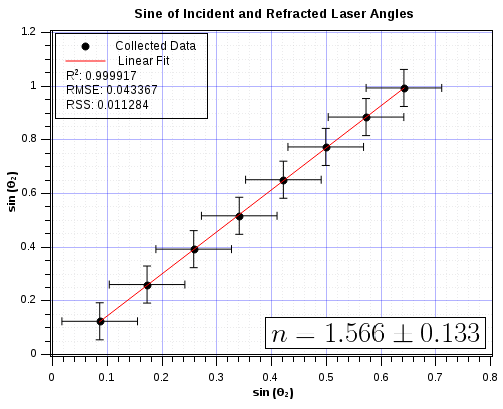
\includegraphics[width=\linewidth]{./graph.png}
	\caption{Linear fit to the ratio of the sines of both angles, giving the ratio of $n_{\text{glass}}$ to $n_{\text{air}}$. Since $n_{\text{air}}$ is taken to be 1, the slope gives the value of $n$ for the glass. }
	\label{fig:graph}
	\end{center}
	\par\end{centering}
\end{figure}

\begin{table}[!H]
\centering{}
\caption{Summary of Refraction Results}
\begin{tabular}{@{}lll@{}}
\toprule
\textbf{Average Index} 		& \textbf{Index from Graph} 	& \textbf{\% Difference} \\ \midrule
1.51$\pm~0.04$           	& 1.5 $\pm~0.1$					& 4\%                      \\ \bottomrule
\end{tabular}
\end{table}
\end{centering}

\subsubsection{Determining Uncertainties}

Since the value for $n$ is constant regardless of the angle of incident light, the averages of the ratios of $\sin\theta_2$ and $\sin\theta_2$ was used as the calculated value of $n$. Since the average should theoretically converge to the true value of $n$, the standard deviation was used as the uncertainty in this calculation.

The plot was generated from the calculated values of the sines of both angles and was fitted with a linear regression to generate a value for $n$. The sine of the uncertainties in instrumental precision were used as error bars for this plot.

\noindent\textit{What can you conclude about the angles formed between the mirror's surface and the light paths?}

In absolute terms, the angle of reflection was extremely close to the angle of incidence. However, relative to one another, the error was more significant.



\section{Questions and Analysis}
\begin{enumerate}
	\item
		\textit{Given the error calculated for the law of reflection, did your result support the conclusion that the angle of incidence equals the angle of reflection?}

		The results show that the angles are very similar, but does not prove that they are necessarily equal.

		The most likely source of the difference between angles is the possibility that the normal lines were not precisely 90 degrees, as the width of the pen marking spanned approximately 0.25$^{\circ}$ on the protractor. It is also possible that minor imperfections on the mirror's surface produced a less than ideal specular reflection -- for example, a slight undulation in the mirror's surface would drastically alter the angle of reflection. Examining the measured data shows that the angle of reflection was slightly lower than the angle of incidence when reflected off of the left hand side of the mirror, and slightly larger when reflected off of the right side. This could indicate slight concavity or convexity of the mirror's surface.
	\item
		\textit{Are the two values obtained for the index of refraction for glass the same? Should they be?}

		Within experimental uncertainty, the values are nearly identical. It is true that this should be the case, as both are derived from the exact same data set. The difference in their value simply arises from the difference between the methods used. In this case, using averages and the standard deviation produced a more precise value. Additionally, both values generally agree with given values for the index of refraction for glass, which ranges between 1.4 and 1.6 for various types.
\end{enumerate}

%\bibliographystyle{plain}
%\bibliography{physbib}

\end{document}